Surrogate models were developed to resolve computational limitations in the analysis of massive datasets by replacing a resource-expensive procedure with a much cheaper approximation
\cite{Sondergaard2003}. They are especially useful in applications where
numerous evaluations of an expensive procedure are required over the same or
similar domains, e.g.~in the parameter optimisation of a theoretical model. The
term ``metamodel'' proves especially meaningful in this case, when the surrogate
model approximates a computational process which is itself a model for a
(perhaps unknown) physical process~\cite{Myers2002}. There exists a spectrum
between ``physical'' surrogates which are constructed with some contextual
knowledge in hand, and ``empirical'' surrogates which are derived purely from
samples of the underlying expensive model.

In this work, we develop an empirical surrogate model for the tritium breeding
ratio (TBR) in an inertial confinement fusion (ICF) reactor. The expensive model
that our surrogate model approximates is a Monte Carlo (MC) neutronics
simulation, Paramak~\cite{paramak}, which returns a prediction of the TBR for a given
configuration of a spherical ICF reactor.

\begin{figure}[!ht]
  \centering
    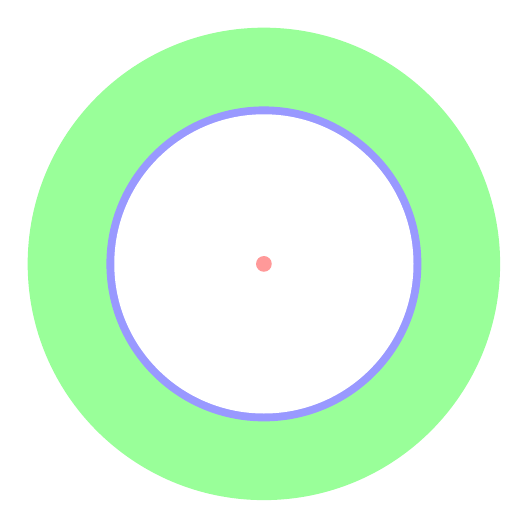
\begin{tikzpicture}
    \fill[green!40!white]  (0,0) circle (3cm);
    \fill[blue!40!white]  (0,0) circle (2cm);
    \fill[white!40!white]  (0,0) circle (1.9cm);
    \fill[red!40!white]  (0,0) circle (0.1cm);
    \end{tikzpicture}

    \caption{Diagram of the simple sphere geometry (not to scale) where the blanket is \fcolorbox{white}{green}{\rule{0pt}{6pt}\rule{6pt}{0pt}}, the first wall is \fcolorbox{white}{blue}{\rule{0pt}{6pt}\rule{6pt}{0pt}} and the neutron point source is \fcolorbox{white}{red}{\rule{0pt}{6pt}\rule{6pt}{0pt}}.}
    \label{fig:model_diagram}
\end{figure}

Paramak facitilates simulation via OpenMC neutronics workflow that is enclosed in
a portable Docker container, which conveniently exposes an HTTP API using the
Python~3 \texttt{flask} package. For the purposes of this work, we used this setup to
simulate a point source with a Muir energy distribution \cite{openmcmuir}
around~\SI{14.06}{\mega\electronvolt} to approximate a Deuterium-Tritium (D-T)
plasma neutron source. Illustrated in~\Fref{fig:model_diagram}, the simulated
geometry was deliberately left tunable, so that dependency of TBR on various
parameters may be investigated.

For the remainder of~\Sref{sec:introduction}, we will define the TBR and further motivate our
research. In~\Sref{sec:methodology} we will present our methodologies for the comparison
testing of a wide variety of surrogate modelling techniques, as well as a novel
adaptive sampling procedure suited to this application. After delivering the
results of these approaches in~\Sref{sec:results}, we will give our final conclusions and
recommendations in~\Sref{sec:conclusion}.


\subsection{Problem Description}
\label{sec:problemdescription}

Nuclear fusion technology relies on the production and containment of an
extremely hot and dense plasma containing enriched Hydrogen isotopes. The current frontier generation of fusion reactors, such as the Joint European Torus (JET) and the
under-construction International Thermonuclear Experimental Reactor (ITER), make
use of both tritium and deuterium fuel. While at least one deuterium atom occurs for every \num{5000} molecules of naturally-sourced water, and may be easily distilled, tritium is extremely rare in nature. It may be produced indirectly through irradiation of heavy water
(\DDO) during nuclear fission, but only at very low rates which could
never sustain industrial-scale fusion power.

Instead, modern D-T reactors rely on tritium breeding blankets, specialised
layers of material which partially line the reactor and produce tritium upon
neutron bombardment, e.g.~by 
\begin{eqnarray}
	\isotope[1][0]{n} + \hspace{3pt} \isotope[6][3]{Li} 
	&\longrightarrow \hspace{3pt} 
	\isotope[3][1]{T} + \hspace{3pt}\isotope[4][2]{He} \\
	\isotope[1][0]{n} + \hspace{3pt} \isotope[7][3]{Li} 
	&\longrightarrow \hspace{3pt} 
	\isotope[3][1]{T} + \hspace{3pt} \isotope[4][2]{He} + \hspace{3pt} \isotope[1][0]{n}
\end{eqnarray}

where T represents tritium and \isotope[7]{Li}, \isotope[6]{Li} are the more and
less common isotopes of lithium, respectively. The TBR is defined as the ratio
between tritium generation in the breeding blanket and consumption in the
reactor, whose description in Paramak is facilitated by 2~classes of parameters
(exhaustively listed in~\Tref{tbl:params}). While the geometry of a given
reactor is described by continuous parameters, material selections are specified
by discrete categorical parameters.

In our work, we set out to produce a fast TBR function which takes these same
input parameters and approximates the MC model used in Paramak with the
greatest achievable regression performance.

\begin{table}[t]
	\setlength\tabcolsep{2pt}
	\renewcommand{\arraystretch}{0.95}
	\caption{\label{tbl:params}Input parameters supplied to Paramak and surrogates in alphabetical order. Groups of fractions marked\textsuperscript{\textdagger
		\textdaggerdbl} are independently required to sum to 1.}
	\begin{indented}
	\item[]
		\begin{tabular}{l|ll}
		\toprule
		{} & Parameter name & Domain\\
		\midrule
		\parbox[t]{2mm}{\hspace{-2pt}\multirow{12}{*}{\rotatebox[origin=c]{90}{Blanket}}}
		   & Breeder fraction\textsuperscript{\textdagger} & $[0,1]$\\
		   & Breeder \isotope[6]{Li} enrichment fraction & $[0,1]$\\
		   & Breeder material & $\{\text{Li}_2\text{TiO}_3, \text{Li}_4\text{SiO}_4\}$\\
		   & Breeder packing fraction & $[0,1]$\\
		   & Coolant fraction\textsuperscript{\textdagger} & $[0,1]$\\
		   & Coolant material & $\{\text{D}_2\text{O}, \text{H}_2\text{O}, \text{He}\}$\\
		   & Multiplier fraction\textsuperscript{\textdagger} & $[0,1]$\\
		   & Multiplier material & $\{\text{Be}, \text{Be}_{12}\text{Ti}\}$\\
		   & Multiplier packing fraction & $[0,1]$\\
		   & Structural fraction\textsuperscript{\textdagger} & $[0,1]$\\
		   & Structural material & $\{\text{SiC}, \text{eurofer}\}$\\
		   & Thickness & $[0,500]$\\
		\midrule
		\parbox[t]{2mm}{\hspace{-2pt}\multirow{6}{*}{\rotatebox[origin=c]{90}{First wall}}}
		   & Armour fraction\textsuperscript{\textdaggerdbl} & $[0,1]$\\
		   & Coolant fraction\textsuperscript{\textdaggerdbl} & $[0,1]$\\
		   & Coolant material & $\{\text{D}_2\text{O}, \text{H}_2\text{O}, \text{He}\}$\\
		   & Structural fraction\textsuperscript{\textdaggerdbl} & $[0,1]$\\
		   & Structural material & $\{\text{SiC}, \text{eurofer}\}$\\
		   & Thickness & $[0,20]$\\
		\bottomrule
		\end{tabular}
	\end{indented}
\end{table}

